\subsection{}
Построим график $d^2_i = F(i)$ для зеленой линии ртути. По наклону прямой
рассчитаем $L$ интерферометра, используя формулу
$$
\frac{\lambda}{L} = \frac{1}{4f^2} \cdot \frac{\Delta (d^2_i)}{\delta (i)}
$$

\begin{figure}[h!]
  \center{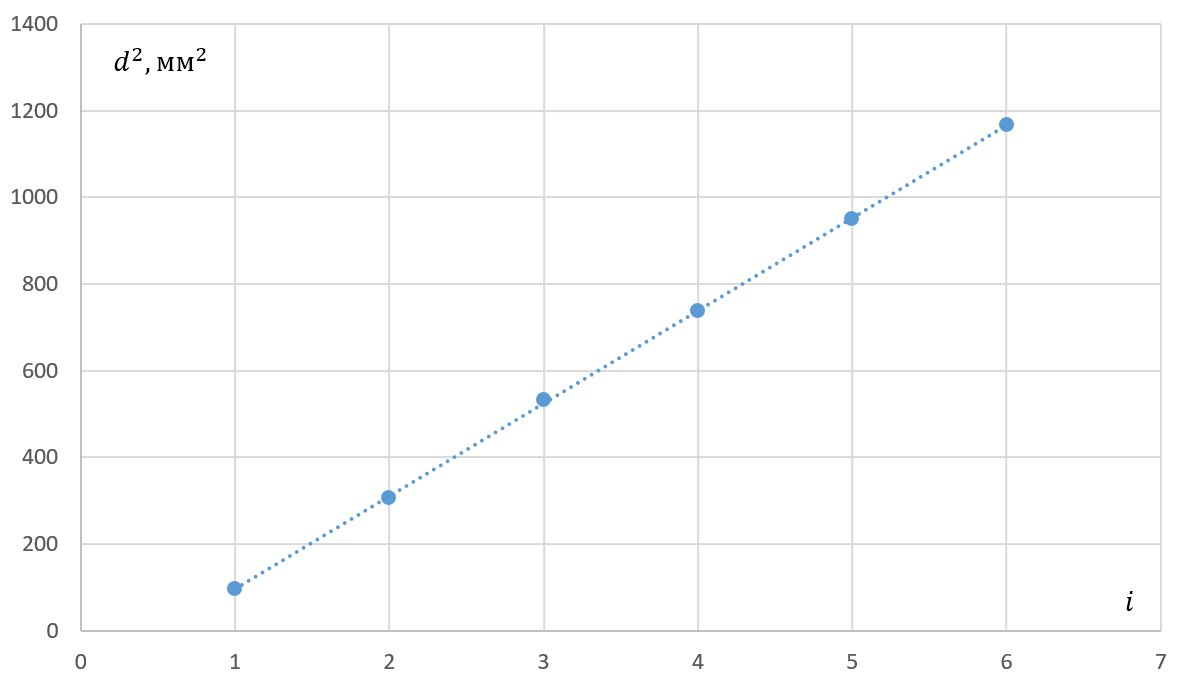
\includegraphics[width=\linewidth]{graph_hg_d_from_i.png}}
  \caption{$d^2_i = F(i)$}
  \label{img::avg_diam_hg}
\end{figure}

Получаем, что для зеленой линии ртути $L = (1.17 \pm 0.01) \cdot 10^{-1}$ мм.

Aналогично для натрия $L = (9.73 \pm 0.11) \cdot 10^{-2}$ мм.

\begin{figure}[h!]
  \center{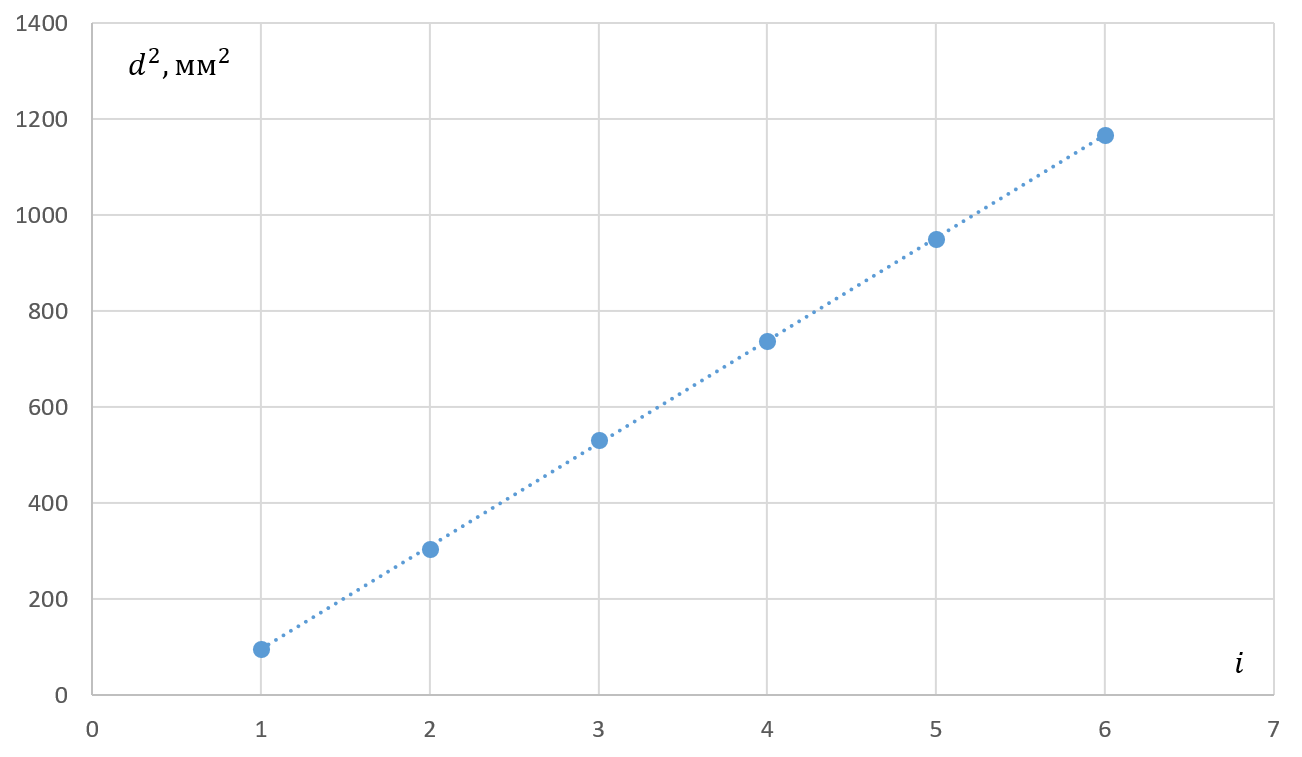
\includegraphics[width=\linewidth]{graph_na_d_from_i.png}}
  \caption{$d^2_i = F(i)$}
  \label{img::avg_diam_na}
\end{figure}

\subsection{}

Найдем зависимость средних диаметров для желтых пар колец Na от разности диаметров
для колец одного порядка. Построим график $\overline{d} = F(1/\Delta d)$ и по
углу его наклона рассчитаем разность длин волн $\Delta \lambda$ для желтой пары
линий ртути

\import{src/}{hg_yellow_circ.tex}

\begin{figure}[h!]
  \center{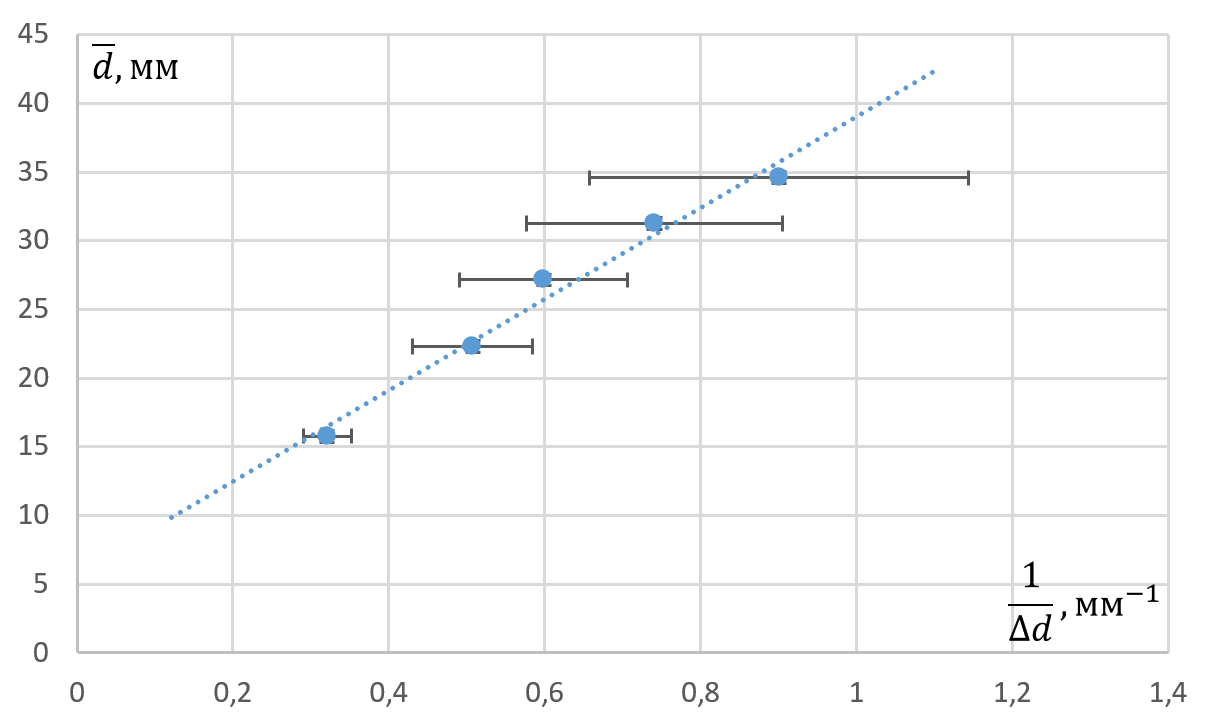
\includegraphics[width=\linewidth]{graph_hg_avd_delta.png}}
  \caption{$\overline{d} = F(1/\Delta d)$}
  \label{img::avg_diam_hg}
\end{figure}

Аналогичную процедуру проведем для натрия.

\begin{table}[h!]
  \begin{center}
    \import{src/}{na.tex}
  \end{center}
  \caption{Измерение диаметров желтых колец натриевой лампы}
\end{table}

\begin{figure}[h!]
  \center{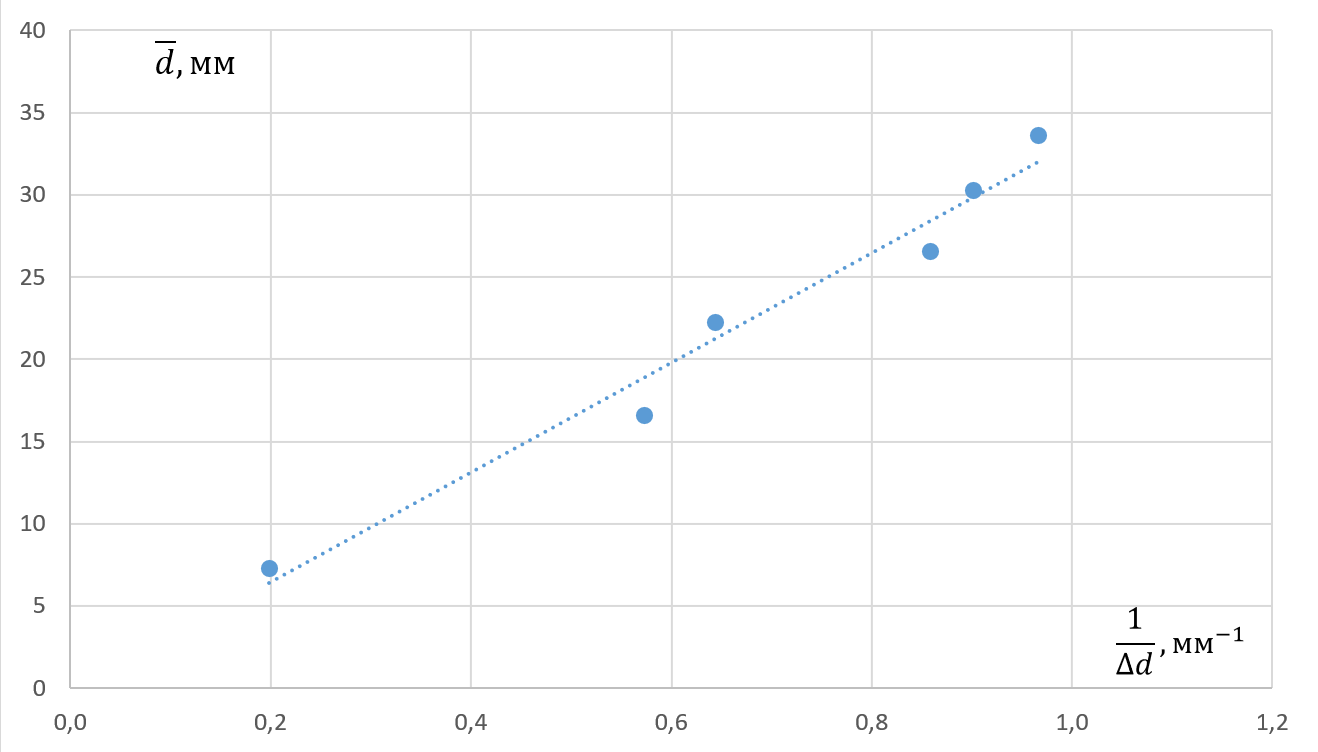
\includegraphics[width=\linewidth]{graph_na_avd_delta.png}}
  \caption{$\overline{d} = F(1/\Delta d)$}
  \label{img::avg_diam_na}
\end{figure}



